% Copyright (C) 2017 - 2019 - Michael Baudin

  \documentclass{beamer}

%\setbeameroption{hide notes}
%\setbeameroption{show notes}
%\setbeameroption{show only notes}

  % Copyright (C) 2012 - 2013 - EDF R&D - Michael Baudin

\setbeameroption{hide notes}
%\setbeameroption{show notes}
%\setbeameroption{show only notes}
%\mode<presentation>{\usetheme{EDF09}}

% Configuration beamer
\usetheme{Montpellier}
\setbeamertemplate{navigation symbols}{} % Remove navigation
\useoutertheme{infolines}
\setbeamertemplate{theorems}[numbered] 
% Utilise des fonts serif, pour �viter les pb de fonte
\usefonttheme{serif} 
\setbeamertemplate{caption}[numbered]


\usepackage[utf8]{inputenc}
\usepackage[T1]{fontenc}


\usepackage[french]{babel}
\uselanguage{French}
\languagepath{French}

% Scilab macros
\newcommand{\sciobj}[1]{\texttt{#1}}
\newcommand{\scifile}[1]{\texttt{#1}}

% Python macros
\newcommand{\pyobj}[1]{\textcolor{blue}{\texttt{#1}}}

\def\RR{\mathbb{R}}
\def\NN{\mathbb{N}}
\def\ZZ{\mathbb{Z}}
\def\bx{{\bf x}}

% To highlight source code
\usepackage{listingsutf8}
\lstset{inputencoding=utf8/latin1}

\definecolor{darkgreen}{rgb}{0,0.5,0}
\definecolor{violet}{rgb}{0.5,0,1}
\lstset{
  % general command to set parameter(s)
   basicstyle=\scriptsize\ttfamily, %
   keywordstyle=\color{violet}\bfseries,%
   commentstyle=\color{darkgreen}\bfseries,%
   showspaces=false,%
   stringstyle=\color{red}\bfseries
}

\hypersetup{
    %bookmarks=true,         % show bookmarks bar?
    %unicode=false,          % non-Latin characters in Acrobat�s bookmarks
    %pdftoolbar=true,        % show Acrobat�s toolbar?
    %pdfmenubar=true,        % show Acrobat�s menu?
    %pdffitwindow=false,     % window fit to page when opened
    %pdfstartview={FitH},    % fits the width of the page to the window
    %pdftitle={My title},    % title
    %pdfauthor={Author},     % author
    %pdfsubject={Subject},   % subject of the document
    %pdfcreator={Creator},   % creator of the document
    %pdfproducer={Producer}, % producer of the document
    %pdfkeywords={keyword1} {key2} {key3}, % list of keywords
    %pdfnewwindow=true,      % links in new window
    colorlinks=true,       % false: boxed links; true: colored links
    %linkcolor=red,          % color of internal links (change box color with linkbordercolor)
    %citecolor=green,        % color of links to bibliography
    %filecolor=magenta,      % color of file links
    urlcolor=blue           % color of external links
}

\title[OpenTURNS]{OpenTURNS and its graphical interface}

\author[Baudin et al.]{
Micha�l Baudin \inst{1} \and
Thibault Delage \inst{1} \and
Anne Dutfoy \inst{1} \and \\
Anthony Geay \inst{1} \and
Ovidiu Mircescu \inst{1} \and
Aur�lie Ladier \inst{2} \and \\
Julien Schueller \inst{2} \and
Thierry Yalamas \inst{2}
}

\institute[EDF-Phim�ca]{
\inst{1} EDF R\&D. 6, quai Watier, 78401, Chatou Cedex - France, michael.baudin@edf.fr \and %
\inst{2} Phimeca Engineering. 18/20 boulevard de Reuilly, 75012 Paris - France, yalamas@phimeca.com
}

\date[]{25 June 2019, UNCECOMP 2019, Crete, Greece}

%%%%%%%%%%%%%%%%%%%%%%%%%%%%%%%%%%%%%%%%%%%%%%%%%%%%%%%%%%%%%%%%%%%%%%%%%%%%%

  \begin{document}

%%%%%%%%%%%%%%%%%%%%%%%%%%%%%%%%%%%%%%%%%%%%%%%%%%%%%%%%%%%%%%%%%%%%%%%%%%%%%

  \begin{frame}
  \titlepage
  
  \begin{columns}
    \column{0.45\textwidth}
  \begin{center}

\includegraphics[height=0.15\textheight]{figures/edf.jpg}
\end{center}
    \column{0.1\textwidth}
	
    \column{0.45\textwidth}
  \begin{center}

\includegraphics[height=0.15\textheight]{figures/logo_phimeca.png}
\end{center}
  \end{columns}

  \end{frame}

\note{
I would like to thank the organizers to inviting us to present our tools. 
}

%%%%%%%%%%%%%%%%%%%%%%%%%%%%%%%%%%%%%%%%%%%%%%%%%%%%%%%%%%%%%%%%%%%%%%%%%%%%%

\begin{frame}
\frametitle{Contents}
\tableofcontents
\end{frame}

%%%%%%%%%%%%%%%%%%%%%%%%%%%%%%%%%%%%%%%%%%%%%%%%%%%%%%%%%%%%%%%%%%%%%%%%%%%%%
\section{Introduction}

%%%%%%%%%%%%%%%%%%%%%%%%%%%%%%%%%%%%%%%%%%%%%%%%%%%%%%%%%%%%%%%%%%%%%%%%%%%%%

\begin{frame}
\frametitle{OpenTURNS: \url{www.openturns.org}}


    \begin{center}
    
\includegraphics[width=0.8\textwidth]{figures/OT.pdf}
    \end{center}
	
\begin{itemize}
\item Multivariate probabilistic modeling including dependence
\item Numerical tools dedicated to the treatment of uncertainties
\item Generic coupling to any type of physical model
\item Open source, LGPL licensed, C++/Python library
\end{itemize}


\end{frame}

\note{
OpenTURNS is a software for uncertainty quantification, uncertainty propagation, 
sensitivity analysis and metamodeling. 

The software is available with the open source LGPL licence on Linux and Windows. 

In order to use OpenTURNS, you can use directly the C++ library, or 
program your Python scripts. 
}
%%%%%%%%%%%%%%%%%%%%%%%%%%%%%%%%%%%%%%%%%%%%%%%%%%%%%%%%%%%%%%%%%%%%%%%%%%%%%

\begin{frame}
\frametitle{OpenTURNS: \url{www.openturns.org}}

\begin{center}
   \begin{tabular}{ccccc}
   
\includegraphics[width=0.07\textwidth]{figures/logoEDF_Anne.png}&
   
\includegraphics[width=0.12\textwidth]{figures/LogoAirbus.png}&
   
\includegraphics[width=0.12\textwidth]{figures/logo_phimeca.png}&
   
\includegraphics[width=0.12\textwidth]{figures/logo_Imacs.png}
   
\includegraphics[width=0.30\textwidth]{figures/logo_ONERA.jpg}&
   \end{tabular}
\end{center}

\vspace*{0.05cm}
\begin{itemize}
\item Linux, Windows
\item First release : 2007
\item 5 full time developers
\item Users $\approx 1000$, mainly in France
(208 000 Total Conda downloads)
\item Project size (2018) : 720 classes, more than 6000 services
\end{itemize}

\end{frame}

\note{
It is developped by five parterns : EDF, Phim�ca, Airbus, IMACS and ONERA.

OpenTURNS was first released in two thousands and seven. 

It is developped by 5 full time developers. 

There are approximately one thousand users worlwide, mainly in France. 

This is a significant software project, with seven hundred classes, 
more than 300 000 (three hundred thousands) lines of codes.
}

%%%%%%%%%%%%%%%%%%%%%%%%%%%%%%%%%%%%%%%%%%%%%%%%%%%%%%%%%%%%%%%%%%%%%%%%%%%%%

\begin{frame}[containsverbatim]
\frametitle{OpenTURNS: content}

    \begin{center}
    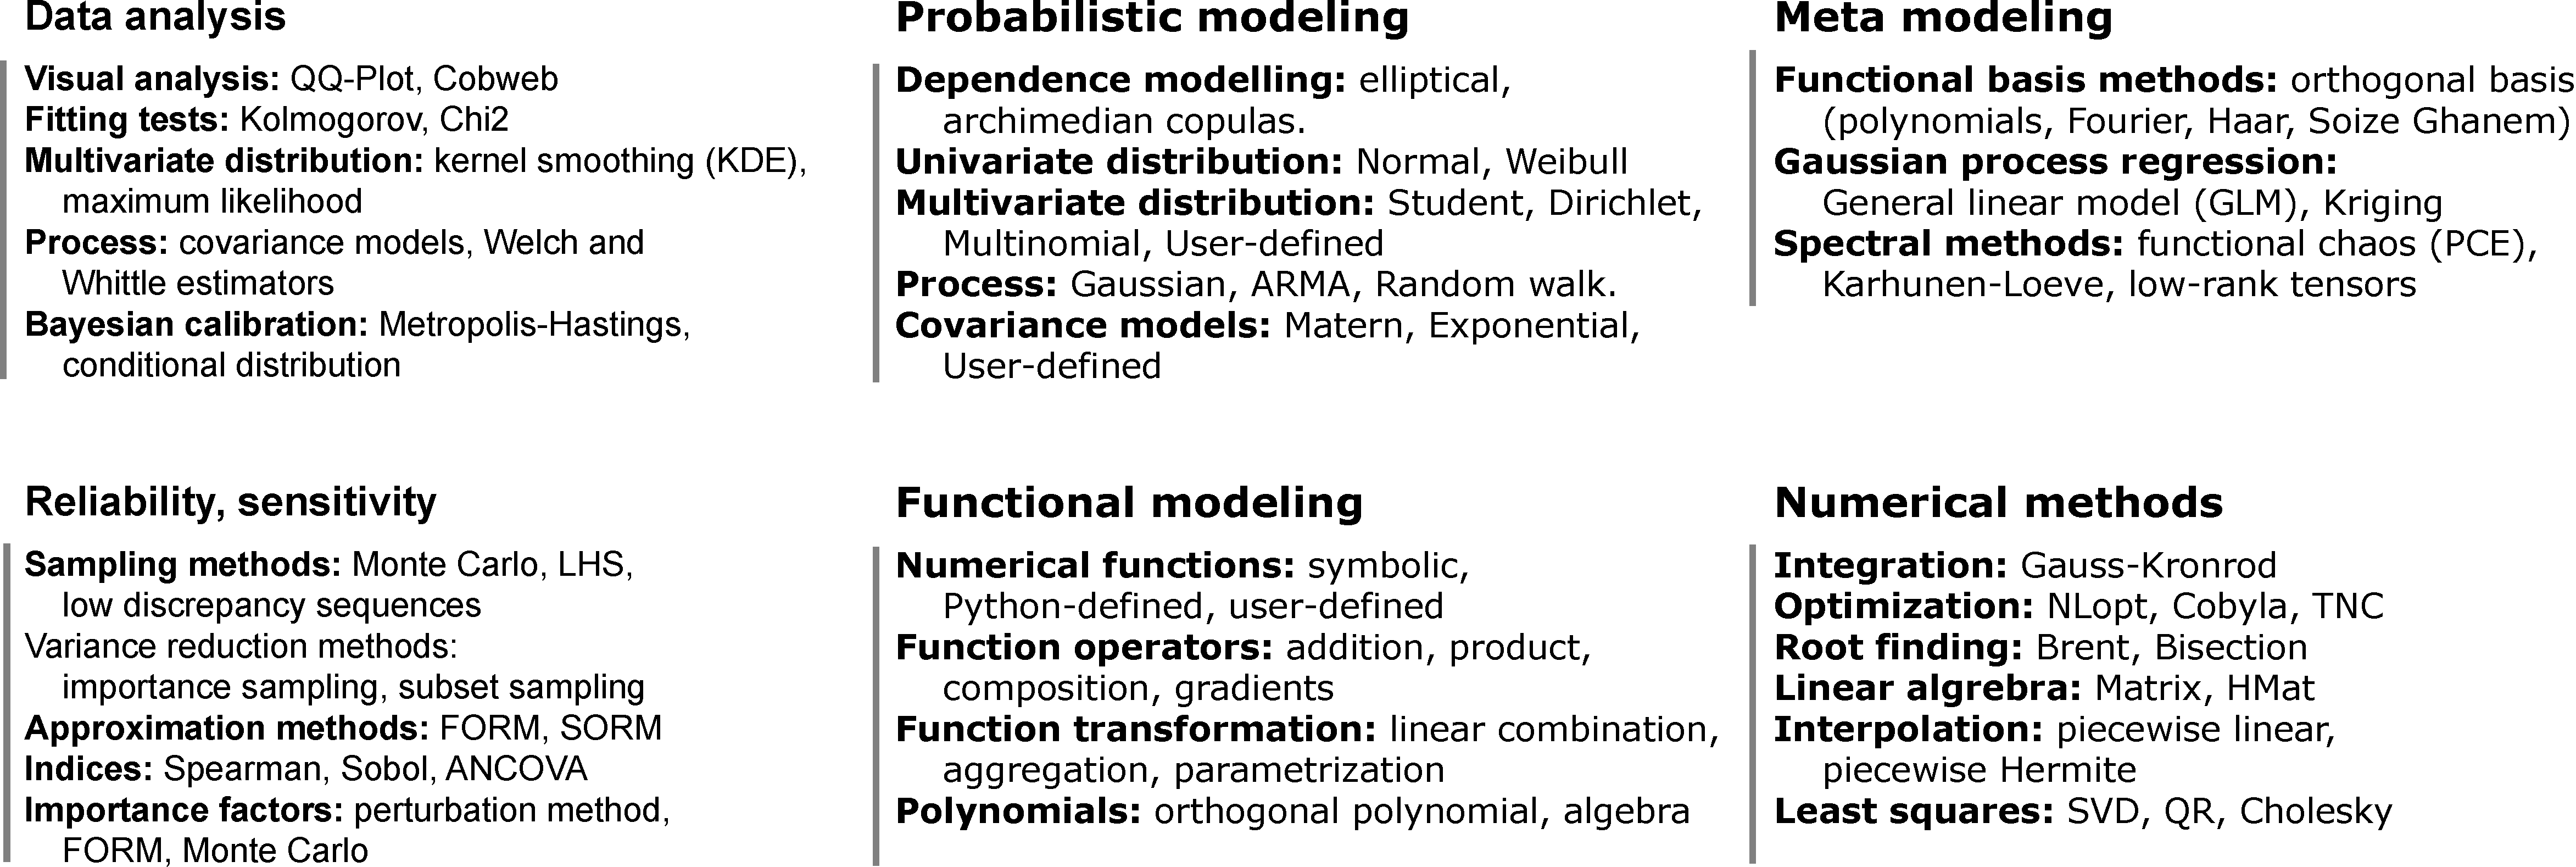
\includegraphics[width=\textwidth]{figures/OpenTURNS-Content-Table.pdf}
    \end{center}

   \begin{tabular}{@{}c@{}c@{}c@{}c@{}c@{}}
   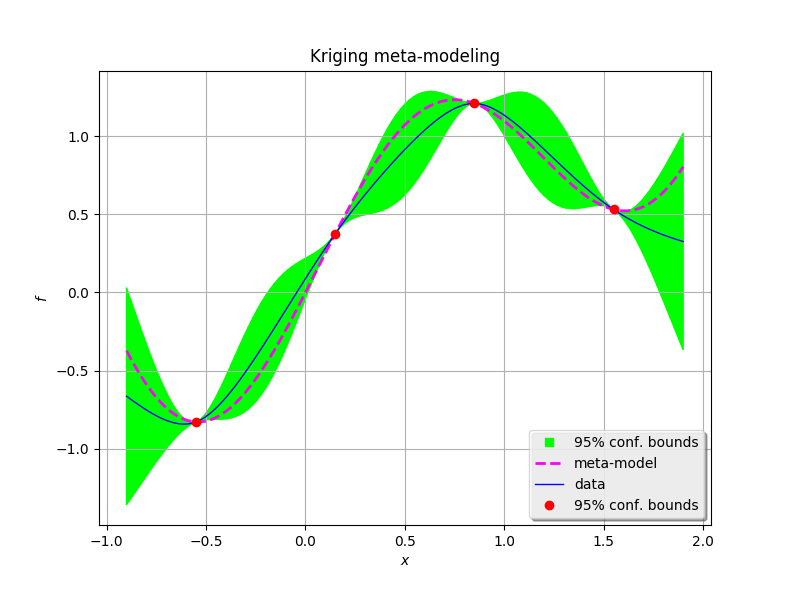
\includegraphics[width=0.2\textwidth]{figures/plot_kriging.png}&
   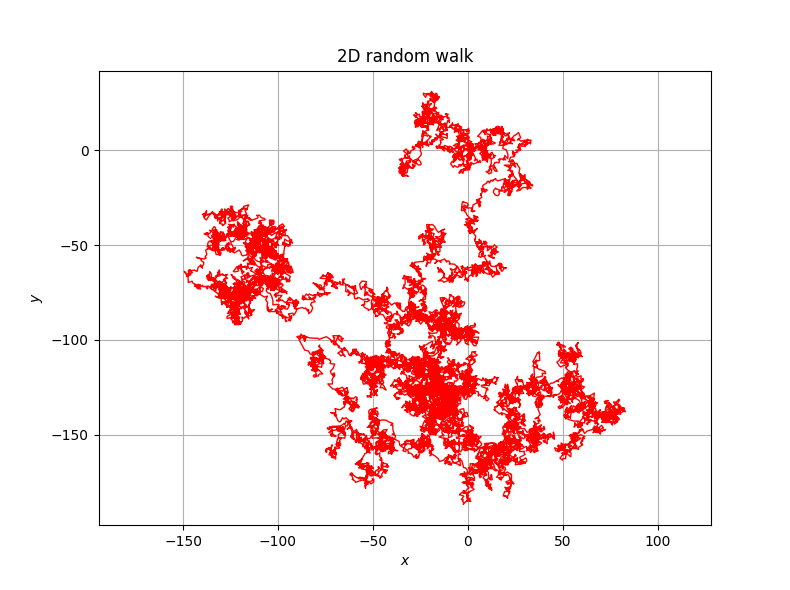
\includegraphics[width=0.2\textwidth]{figures/plot_random_walk.png}&
   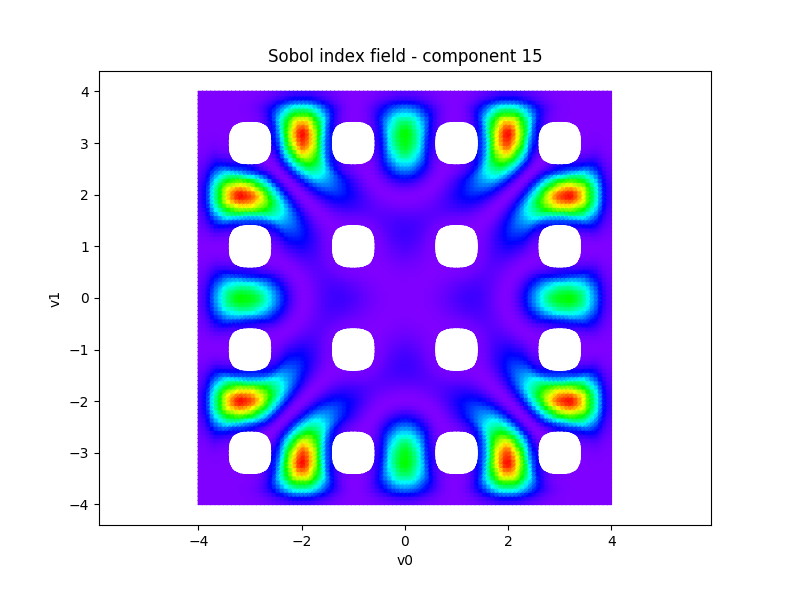
\includegraphics[width=0.2\textwidth]{figures/plot_sobol_field.png}&
   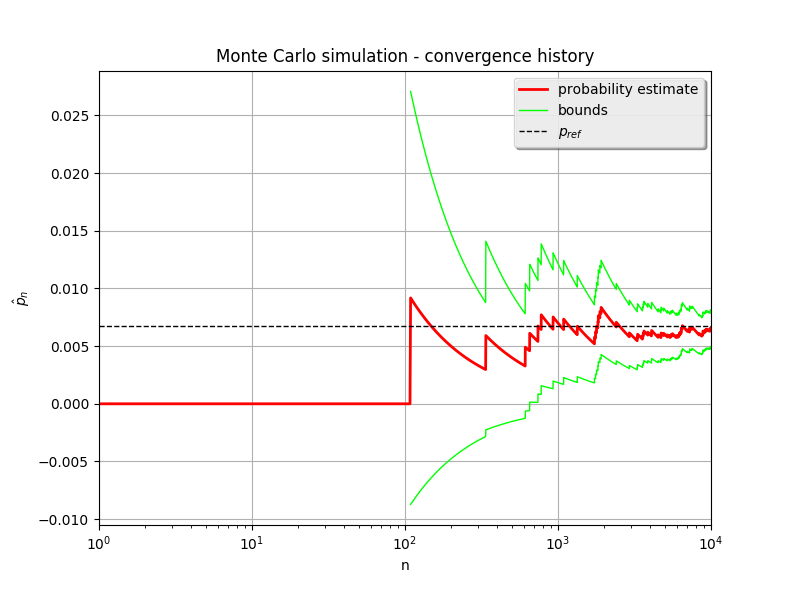
\includegraphics[width=0.2\textwidth]{figures/plot_monte_carlo.png}&
   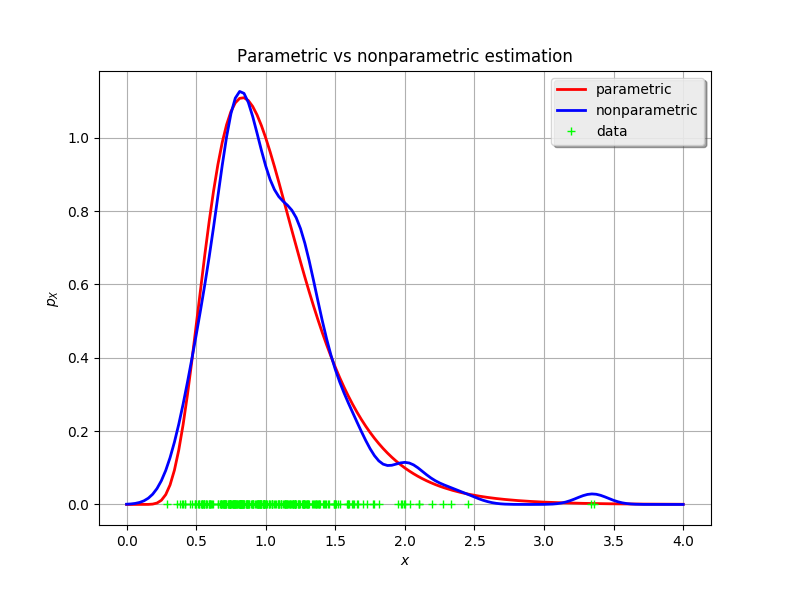
\includegraphics[width=0.2\textwidth]{figures/plot_distribution_fitting.png}
   \end{tabular}
\end{frame}


\note{
This is a global picture of the main features: data analysis, 
probabilistic modeling, meta-modeling, reliability, sensitivity analysis, 
functional modeling and numerical methods, and, of course, graphics. 
}

%%%%%%%%%%%%%%%%%%%%%%%%%%%%%%%%%%%%%%%%%%%%%%%%%%%%%%%%%%%%%%%%%%%%%%%%%%%%%

\begin{frame}[containsverbatim]
\frametitle{OpenTURNS: documentation}

\small{

\begin{columns}
    \column{0.5\textwidth}

    \begin{center}
    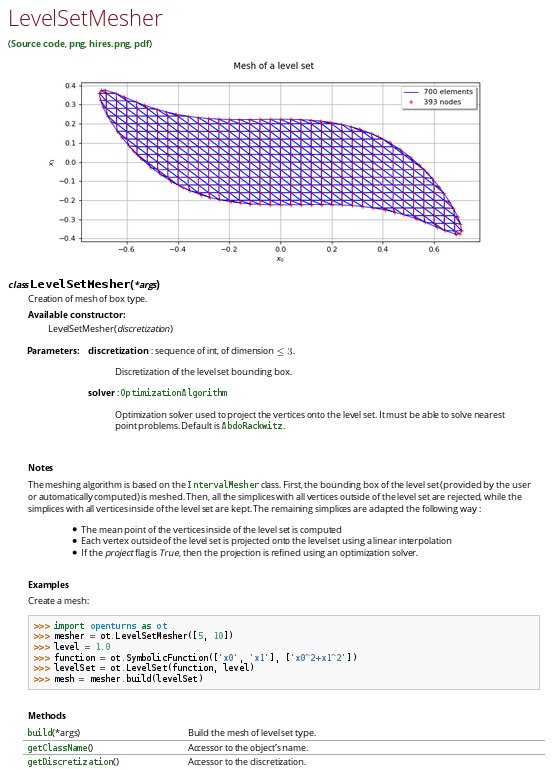
\includegraphics[width=0.8\textwidth]{figures/exClasses.png}
    \end{center}

    \column{0.5\textwidth}

    \begin{center}
    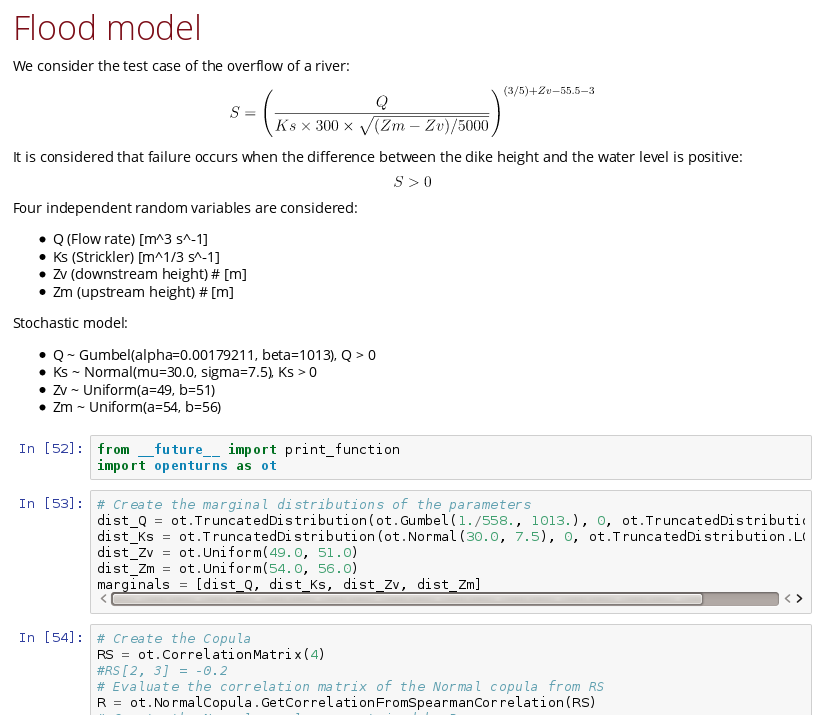
\includegraphics[width=0.9\textwidth]{figures/exRefGuide.png}
    \end{center}
	
\end{columns}

}
\end{frame}

\note{
The documentation is available online with a technical documentation of the 
programming interface, that is to say, the classes (for example the 
LevelSetMesher class) with a description of the arguments and small examples (the 
examples are automatically tested). 

The documentation also provide larger examples and a theoretical documentation. 
}

% %%%%%%%%%%%%%%%%%%%%%%%%%%%%%%%%%%%%%%%%%%%%%%%%%%%%%%%%%%%%%%%%%%%%%%%%%%%%%

\section{Sequential algorithms}

% %%%%%%%%%%%%%%%%%%%%%%%%%%%%%%%%%%%%%%%%%%%%%%%%%%%%%%%%%%%%%%%%%%%%%%%%%%%%%

\begin{frame}[containsverbatim]
\frametitle{OpenTURNS: estimate the mean sequentially}

Two sequential algorithms based on asymptotic statistics: the mean 
and Sobol' sensitivity indices.


Part 1 : Estimate the mean with an sequential algorithm.
\begin{itemize}
\item The "classical" way of estimating the mean : set the sample size $n$, 
then use the sample mean $\mu = (1/n) \sum_{j=1}^n y^{(j)}$.

\item The sample mean is asymptotically gaussian:
$$
\mu \rightarrow \mathcal{N}\left(E(Y),\frac{V(Y)}{n}\right).
$$

\item The absolute precision of the estimate $\mu$ can be evaluated based on the sample
standard deviation of the estimator $\frac{s}{\sqrt{n}}$ 
%where $s$ is the unbiased sample standard deviation of the output.

\item To set the relative precision, we can consider the coefficient of variation 
of the estimator (if $E(Y)\neq 0$).

\item To get good performances on distributed supercomputers and 
multi-core workstations, the size of the sample increases by block.

\end{itemize}

\end{frame}


\note{
I would now like to introduce two new sequential algorithms which are new in OT 1.12. 

These algorithms are based on asymptotic statistics. 

Part 1 is on estimating the mean and part 2 is on sensitivity indices. 

Suppose that you want to estimate the mean of a random variable $Y$, where 
$Y$ is the output of a computer code. 

Assume that there is only one single output (it is easy to generalize this 
to multiple outputs).
}

% %%%%%%%%%%%%%%%%%%%%%%%%%%%%%%%%%%%%%%%%%%%%%%%%%%%%%%%%%%%%%%%%%%%%%%%%%%%%%

\begin{frame}[containsverbatim]
\frametitle{OpenTURNS: estimate the mean sequentially}

\scriptsize{

\lstset{language=python}
\begin{lstlisting}
[... Define the Y RandomVector ...]
algo = ot.ExpectationSimulationAlgorithm(Y)
algo.setMaximumOuterSampling(1000)
algo.setBlockSize(10)
algo.setMaximumCoefficientOfVariation(0.001)
algo.run()
result = algo.getResult()
expectation = result.getExpectationEstimate()
print("Mean = %f " % expectation[0])
meanDistr = result.getExpectationDistribution()
View(meanDistr.drawPDF())
\end{lstlisting}

\begin{lstlisting}
Mean = -5.972516 
\end{lstlisting}

}

	\begin{center}
	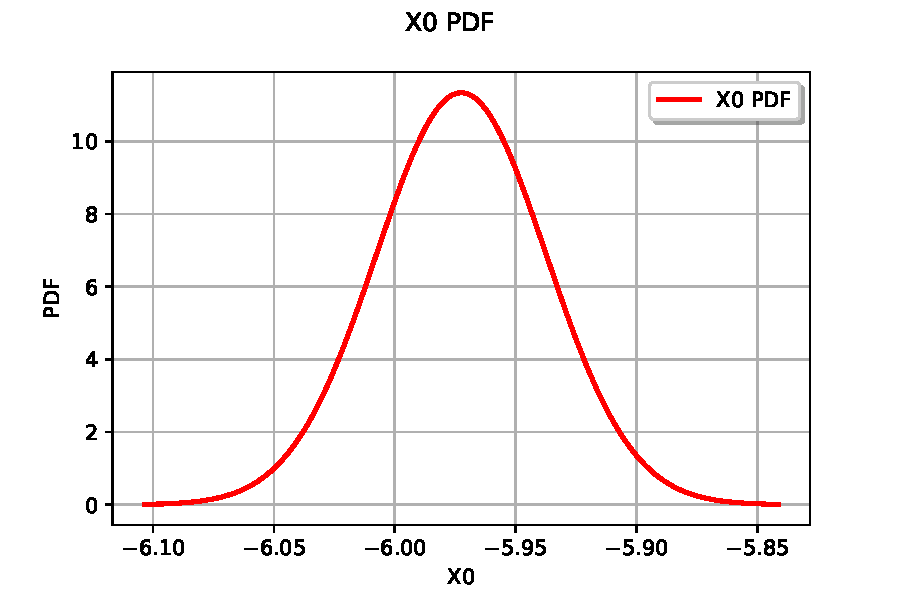
\includegraphics[width=0.3\textwidth]{figures/MeanDistribution.pdf}
	\end{center}
Asymptotic distribution of the sample mean.


\end{frame}

\note{
We use the ExpectationSimulationAlgorithm class. 

We set the setMaximumOuterSampling to 1000 (one thousands). This is the 
number of outer iterations. 

We set the setBlockSize to 10 (ten). This is the 
block size (i.e. the number of inner iterations). 

To define the stopping criteria, we set the setMaximumCoefficientOfVariation 
to 0.001 (point zero zero one). 

And we run. 

The getResult method returns an object that contains the result of the 
algorithm. 
The getExpectationEstimate returns the estimated mean. 

Most importantly, the getExpectationDistribution method returns the gaussian 
distribution, that we can plot. 
We can, if required, derive a 95\% confidence interval. 
}
% %%%%%%%%%%%%%%%%%%%%%%%%%%%%%%%%%%%%%%%%%%%%%%%%%%%%%%%%%%%%%%%%%%%%%%%%%%%%%

\begin{frame}[containsverbatim]
\frametitle{OpenTURNS: estimate Sobol' indices sequentially}

Part 2 : Estimate Sobol' sensitivity indices with an incremental algorithm.
\begin{itemize}
\item Assume that the Sobol' estimator is 
$$
\overline{S} = \Psi\left(\overline{U}\right)
$$
where $\Psi$ is a multivariate function, $U$ is a multivariate sample and $\overline{U}$ is its 
sample mean. 

\item Each Sobol' estimator (e.g. Saltelli, Jansen, etc...) 
can be associated with a specific choice of function $\Psi$ and vector $U$. 

\item Therefore, the multivariate delta method implies:
$$
\sqrt{n} \left(\overline{U} - \mu\right) \rightarrow \mathcal{N}\left(0,\nabla \psi(\mu)^T \Gamma\nabla \psi(\mu)\right)
$$
where $\mu$ is the expected value of the Sobol' indice, $\nabla \psi(\mu)$ is the 
gradient of the function $\Psi$ and $\Gamma$ is the covariance matrix of 
$\overline{U}$. 

\item An implementation of the exact gradient $\nabla \psi(\mu)$ was 
derived for all estimators in OpenTURNS.  

\end{itemize}

\end{frame}

\note{
We did the same to estimate the sensitivity indices. 

The trick is to define the Sobol' estimator as follows ... 
where $\Psi$ is a multivariate function, 
$U$ is a multivariate sample and $\overline{U}$ is its 
sample mean. 

}

% %%%%%%%%%%%%%%%%%%%%%%%%%%%%%%%%%%%%%%%%%%%%%%%%%%%%%%%%%%%%%%%%%%%%%%%%%%%%%

\begin{frame}[containsverbatim]
\frametitle{OpenTURNS: estimate Sobol' indices sequentially}

Part 2 : Estimate Sobol' sensitivity indices with an incremental algorithm.
\begin{itemize}
\item Let us denote by $\Phi_k^F$ (resp. $\Phi_k^T$) the cumulated 
distribution function of the gaussian distribution of the first (resp. total) 
order sensitivity indice of the k-th input variable.

\item We set $\alpha\in[0,1]$ a quantile level and $\epsilon \in(0,1]$ a quantile precision. 

\item The algorithms stops when, on all components, first and total order 
indices haved been estimated with enough precision.
 
The precision is said to be sufficient if 
$$
\Phi_k^F(1-\alpha) - \Phi_k^F(\alpha) \leq \epsilon
$$
and 
$$
\Phi_k^T(1-\alpha) - \Phi_k^T(\alpha) \leq \epsilon
$$
for $k=1,...,n_X$. 

\end{itemize}

\end{frame}

\note{
We now define the stopping criteria. 
}


%%%%%%%%%%%%%%%%%%%%%%%%%%%%%%%%%%%%%%%%%%%%%%%%%%%%%%%%%%%%%%%%%%%%%%%%%%%%%

% %%%%%%%%%%%%%%%%%%%%%%%%%%%%%%%%%%%%%%%%%%%%%%%%%%%%%%%%%%%%%%%%%%%%%%%%%%%%%

\begin{frame}[containsverbatim]
\frametitle{OpenTURNS: estimate Sobol' indices sequentially}

\scriptsize{

\lstset{language=python}
\begin{lstlisting}
[... Define the X Distribution, define the g Function...]
estimator = ot.SaltelliSensitivityAlgorithm()
estimator.setUseAsymptoticDistribution(True)
algo = ot.SobolSimulationAlgorithm(X, g, estimator)
algo.setMaximumOuterSampling(100) # number of iterations
algo.setBlockSize(50)  # size of Sobol experiment at each iteration
algo.setBatchSize(16) # number of points evaluated simultaneously
# alpha, the confidence interval level
algo.setIndexQuantileLevel(0.1) 
# epsilon, a quantile precision
algo.setIndexQuantileEpsilon(0.2) 
algo.run()
\end{lstlisting}

}

	\begin{center}
	\includegraphics[width=0.3\textwidth]{figures/S0-Distribution.pdf}
	\end{center}
Asymptotic distribution of the first order Sobol' indices for the first variable.

\end{frame}


\note{
We use the SaltelliSensitivityAlgorithm class to define the 
sensitivity estimator. 

The sequential algorithm is provided by the SobolSimulationAlgorithm class. 

We set the setMaximumOuterSampling, which is the number of outer 
iterations. 

We set the block size with setBlockSize (i.e. the size of the 
inner iterations). 

Then the setIndexQuantileLevel sets the confidence interval level 
and the setIndexQuantileEpsilon sets the confidence interval length. 
}

% %%%%%%%%%%%%%%%%%%%%%%%%%%%%%%%%%%%%%%%%%%%%%%%%%%%%%%%%%%%%%%%%%%%%%%%%%%%%%

\section{PERSALYS, the graphical user interface}

\begin{frame}
\frametitle{SALOME}

  \begin{columns}
    \column{0.5\textwidth}
	
\begin{itemize}
\item Integration platform for pre and post processing, and 2D/3D numerical simulation 
\item Features : geometry, mesh, distributed computing
\item Visualization, data assimilation, uncertainty treatment
\item Partners : EDF, CEA, Open Cascade
\item Licence : LGPL
\item Linux, Windows
\item \url{www.salome-platform.org}
\end{itemize}

    \column{0.5\textwidth}

\begin{center}
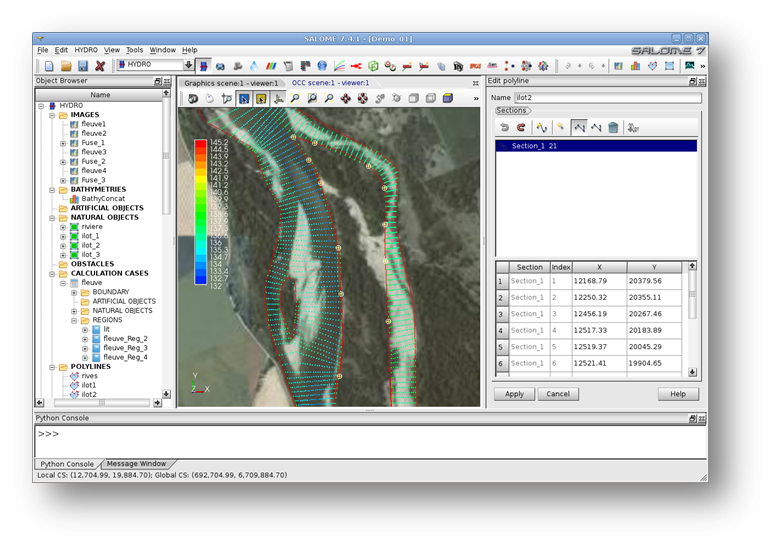
\includegraphics[width=0.95\textwidth]{figures/Salome-hydro-platform}
\end{center}

	\end{columns}
\end{frame}

\note{
Before presenting the graphical user interface, I would like to say some 
words about SALOME.
}

%%%%%%%%%%%%%%%%%%%%%%%%%%%%%%%%%%%%%%%%%%%%%%%%%%%%%%%%%%%%%%%%%%%%%%%%%%%%%

\begin{frame}
\frametitle{PERSALYS, the graphical user interface of \ot{}}
	
\begin{itemize}
\item Main goal : provide a graphical interface of 
\ot{} in SALOME
\item Features
	\begin{itemize}
	\item Uncertainty quantification : definition of the 
	probabilistic model (including dependence), distribution fitting (including 
	copulas), central tendency, sensitivity analysis, probability estimate, 
	meta-modeling (polynomial chaos, kriging), screening with Morris, 
	optimization, design of experiments
	\item Generic (not dedicated to a specific application)
	\item GUI language : English, French
	\end{itemize}

\item Partners : EDF, Phim�ca
\item Licence : LGPL

\item Schedule : 
	\begin{itemize}
	\item Since summer 2016, one EDF release per year
	\item On the internet (free) : SALOME\_EDF since 2018 on 
	
	\url{https://www.salome-platform.org}
	
	
	\end{itemize}

\end{itemize}

\end{frame}

\note{
We created a new tool within SALOME, called PERSALYS. 
}

%%%%%%%%%%%%%%%%%%%%%%%%%%%%%%%%%%%%%%%%%%%%%%%%%%%%%%%%%%%%%%%%%%%%%%%%%%%%%

\begin{frame}
\frametitle{PERSALYS: define the dependence}
	

  \begin{columns}
    \column{0.4\textwidth}
	
\begin{itemize}
\item Dependence is defined using copulas
\item Define arbitrary groups of dependent variables
\item Available copulas (same as in OT): gaussian, Ali-Mikhail-Haq, 
    Clayton, Farlie-Gumbel-Morgenstern, Frank, Gumbel
\end{itemize}

    \column{0.6\textwidth}

\begin{center}
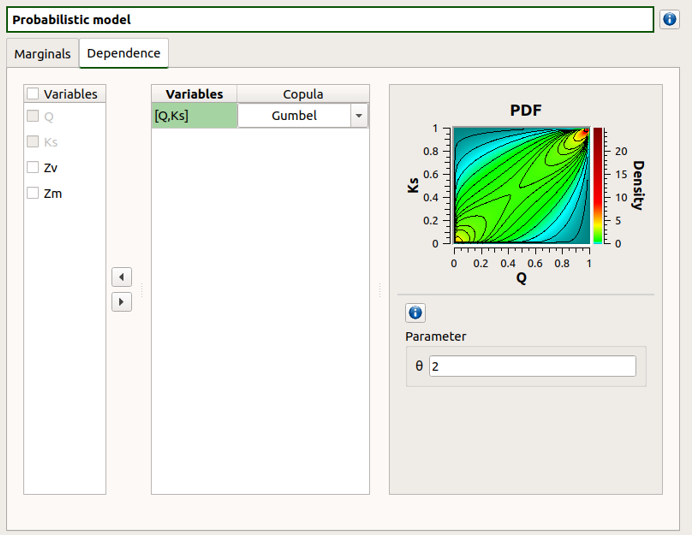
\includegraphics[width=0.95\textwidth]{figures/persalys-dependence-extract.png}
\end{center}

	\end{columns}

\end{frame}

\note{
To define the dependence in PERSALYS, we use the copula tools available in OpenTURNS. 

The Dependence tab shows the list of input variables: you can create a group 
of dependent variables using the checkbutton and add it to the group. 
}

%%%%%%%%%%%%%%%%%%%%%%%%%%%%%%%%%%%%%%%%%%%%%%%%%%%%%%%%%%%%%%%%%%%%%%%%%%%%%

\begin{frame}
\frametitle{PERSALYS: estimate the parameters of the copulas}
	

  \begin{columns}
    \column{0.4\textwidth}
	
\begin{itemize}
\item Inference of the dependence of the multivariate sample 
\item Guided choice according to the BIC and Kendall plot
\end{itemize}

    \column{0.6\textwidth}

\begin{center}
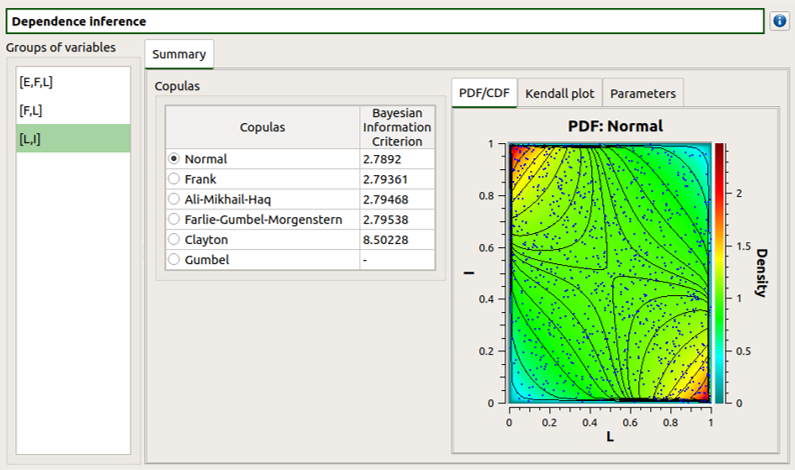
\includegraphics[width=0.95\textwidth]{figures/persalys-copula-inference.png}
\end{center}

	\end{columns}


\end{frame}

\note{
To estimate the parameters of a copula, you can perform the inference of a 
multivariate sample. 
}

%%%%%%%%%%%%%%%%%%%%%%%%%%%%%%%%%%%%%%%%%%%%%%%%%%%%%%%%%%%%%%%%%%%%%%%%%%%%%

\begin{frame}
\frametitle{PERSALYS: 1D fields}
	

\begin{itemize}
\item Mesh definition and visualization
\item Import from text or csv file
\end{itemize}

\begin{center}
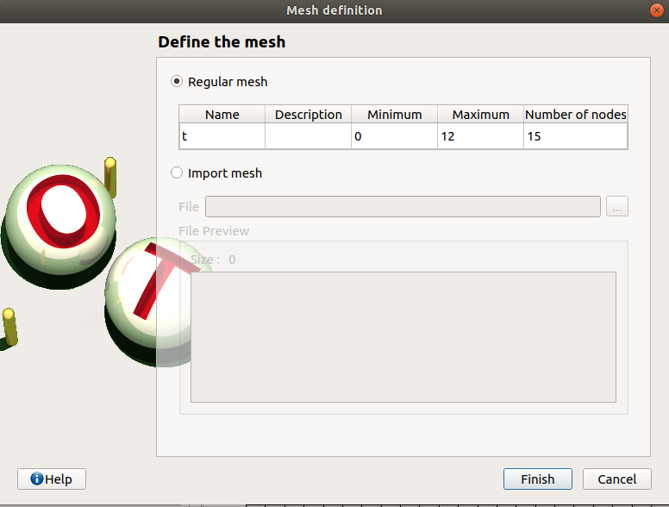
\includegraphics[width=0.45\textwidth]{figures/persalys-field-define-mesh.png}
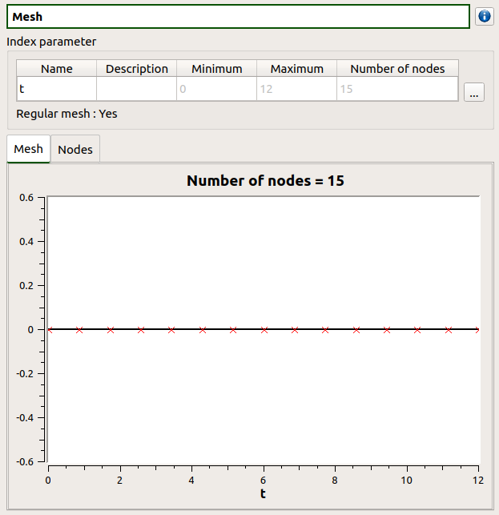
\includegraphics[width=0.45\textwidth]{figures/persalys-field-visualize-mesh-extract.png}
\end{center}

\end{frame}

\note{
The most important new feature is the management of 1D stochastic processes. 


}

%%%%%%%%%%%%%%%%%%%%%%%%%%%%%%%%%%%%%%%%%%%%%%%%%%%%%%%%%%%%%%%%%%%%%%%%%%%%%

\begin{frame}
\frametitle{PERSALYS: 1D fields}
	
\begin{itemize}
\item Functional model definition and probabilistic model
\item Python or symbolic
\end{itemize}

\begin{center}
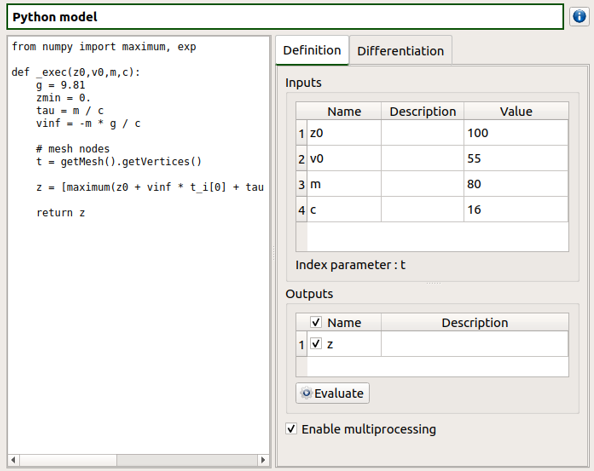
\includegraphics[width=0.45\textwidth]{figures/persalys-field-define-python-model-extract.png}
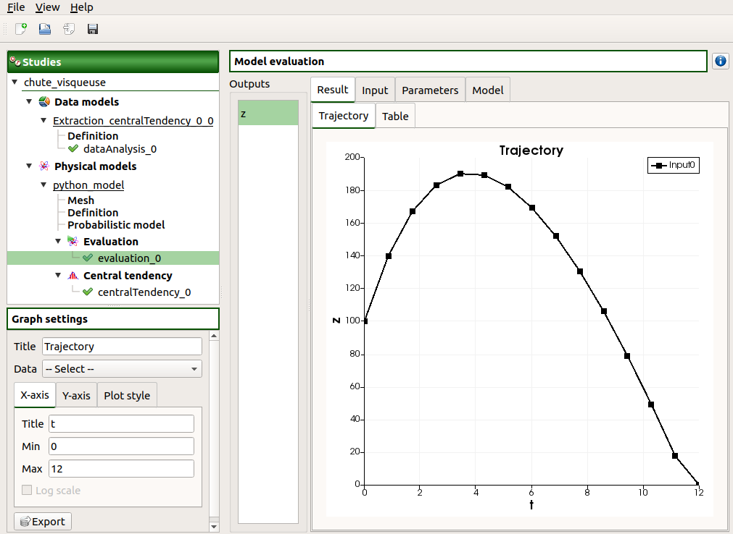
\includegraphics[width=0.45\textwidth]{figures/persalys-field-evaluation.png}
\end{center}

\end{frame}

\note{
The Python function has 4 (four) inputs named z0, v0, m and c. 

Moreover, the Python function depends on the index parameter which name is "t". 

On the right figure, this is what appears when we click on the "Evaluate" button: 
one evaluation of the function is then a trajectory which depends on the time. 
}

%%%%%%%%%%%%%%%%%%%%%%%%%%%%%%%%%%%%%%%%%%%%%%%%%%%%%%%%%%%%%%%%%%%%%%%%%%%%%

\begin{frame}
\frametitle{PERSALYS: 1D fields}
	
\begin{itemize}
\item Probabilistic model
\item Uncertainty propagation with simple Monte-Carlo sampling
\end{itemize}

\begin{center}
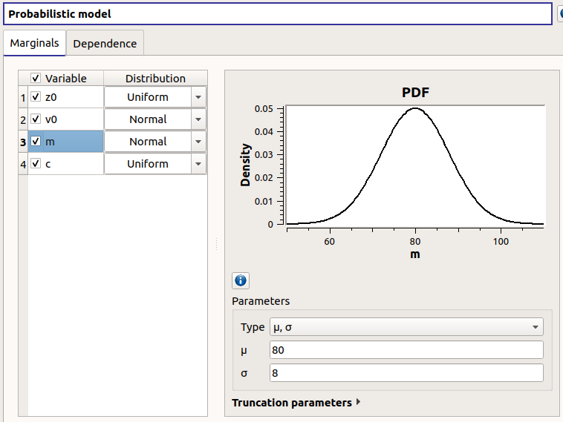
\includegraphics[width=0.45\textwidth]{figures/persalys-field-probabilistic-model.png}
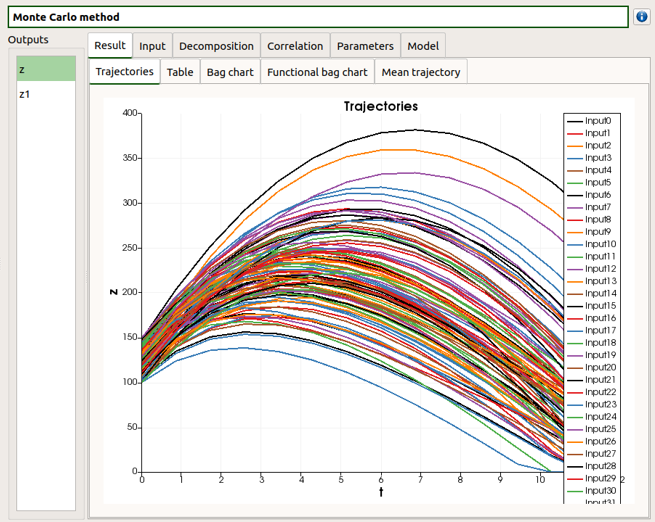
\includegraphics[width=0.45\textwidth]{figures/persalys-field-montecarlo-trajectories-extract.png}
\end{center}

\end{frame}

\note{
Then we can perform the central dispersion analysis of the model. 

On the left, we define the distribution of the input random vector. 

On the right, this is the result of the simulation: a sample made 
of 100 (one hundred) trajectories. 
}
%%%%%%%%%%%%%%%%%%%%%%%%%%%%%%%%%%%%%%%%%%%%%%%%%%%%%%%%%%%%%%%%%%%%%%%%%%%%%

\begin{frame}
\frametitle{PERSALYS: 1D fields}
	
\begin{itemize}
\item BagChart and Functional Bagchart (from Paraview) 
based on High Density Regions.
\item To do this, Paraview uses OpenTURNS to perform the Karhunen-Lo�ve 
decomposition. 
\item Linked selections in the views
\end{itemize}

\begin{center}
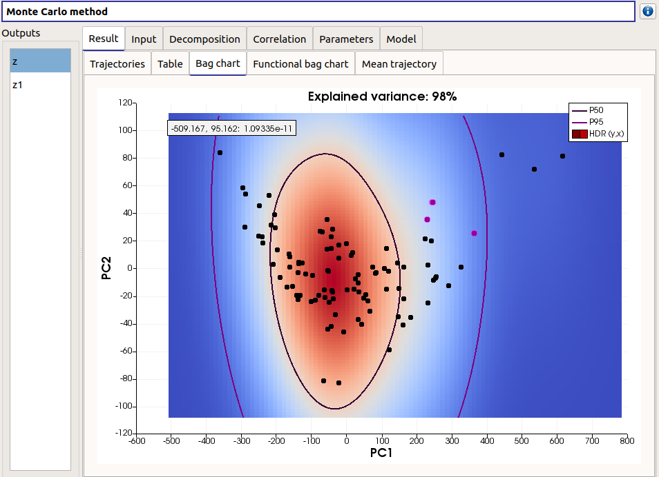
\includegraphics[width=0.45\textwidth]{figures/persalys-field-bagchart.png}
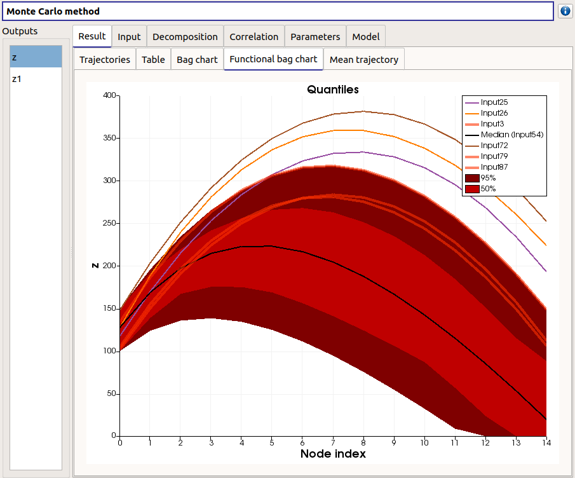
\includegraphics[width=0.45\textwidth]{figures/persalys-field-functional-bagchart.png}
\end{center}

\end{frame}

\note{
To analyze these trajectories requires more advanced tools than with 
classical multivariate samples, so that we can take into account for the 
time dependence. 

We use the BagChart and Functional Bagchart (from Paraview) tools, 
which uses the High Density Regions algorithm (Hyndman, 1996). 
}


%%%%%%%%%%%%%%%%%%%%%%%%%%%%%%%%%%%%%%%%%%%%%%%%%%%%%%%%%%%%%%%%%%%%%%%%%%%%%
\section{What's next ?}


\begin{frame}
\frametitle{What's next ?}
  \begin{columns}
    \column{0.5\textwidth}

PERSALYS Roadmap : 
\begin{itemize}
\item Calibration
\item 2D Fields, 3D Fields
\item In-Situ fields based on the MELISSA library (with INRIA)
\end{itemize}

    \column{0.5\textwidth}

\begin{center}
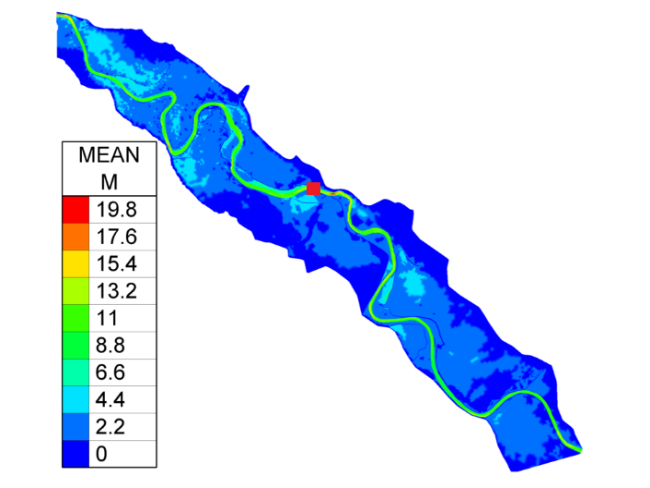
\includegraphics[height=0.5\textheight]{figures/image034.png}
\end{center}

	\end{columns}

\end{frame}

\note{
We are currently working on adding features to perform 
the calibration of a computer code (almost done). 

The next features we plan to add to PERSALYS are the management 
of 2D and 3D stochastic fields. 

We also work on the use of the MELISSA software which performs 
in-situ studies. 

This library allows to perform UQ studies in situations 
where we cannot store more than a couple of multidimensional fields 
in memory or on the hard drive. 
}

%%%%%%%%%%%%%%%%%%%%%%%%%%%%%%%%%%%%%%%%%%%%%%%%%%%%%%%%%%%%%%%%%%%%%%%%%%%%%

\begin{frame}
\frametitle{The end}

\begin{center}
Thanks !
\end{center}

\begin{center}
Questions ?
\end{center}

\end{frame}

\note{
Thank you for your attention. 

If you have any question, it would be a pleasure to answer them. 

If you want a live demo of PERSALYS, I can show you during the coffee break.
}
%%%%%%%%%%%%%%%%%%%%%%%%%%%%%%%%%%%%%%%%%%%%%%%%%%%%%%%%%%%%%%%%%%%%%%%%%%%%%

\begin{frame}
\frametitle{PERSALYS: 1D fields}
	
\begin{itemize}
\item Karhunen Loeve decomposition
\item Show modes, eigenvalues and projection coefficients
\end{itemize}

\begin{center}
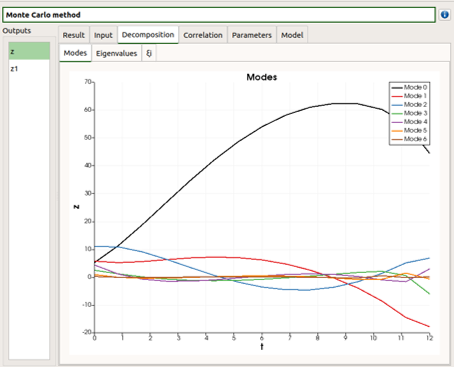
\includegraphics[width=0.45\textwidth]{figures/persalys-field-modes.png}
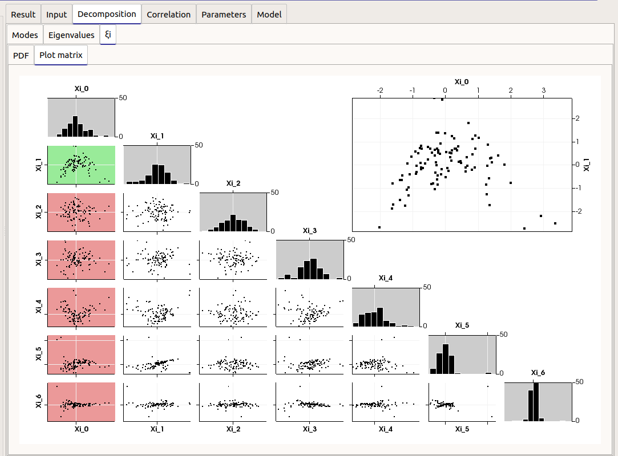
\includegraphics[width=0.45\textwidth]{figures/persalys-field-plotmatrix-extract.png}
\end{center}

\end{frame}
%%%%%%%%%%%%%%%%%%%%%%%%%%%%%%%%%%%%%%%%%%%%%%%%%%%%%%%%%%%%%%%%%%%%%%%%%%%%%
%\section{Extra slides}

\begin{frame}
\frametitle{Interactive uncertainty visualization with Paraview}

\begin{center}
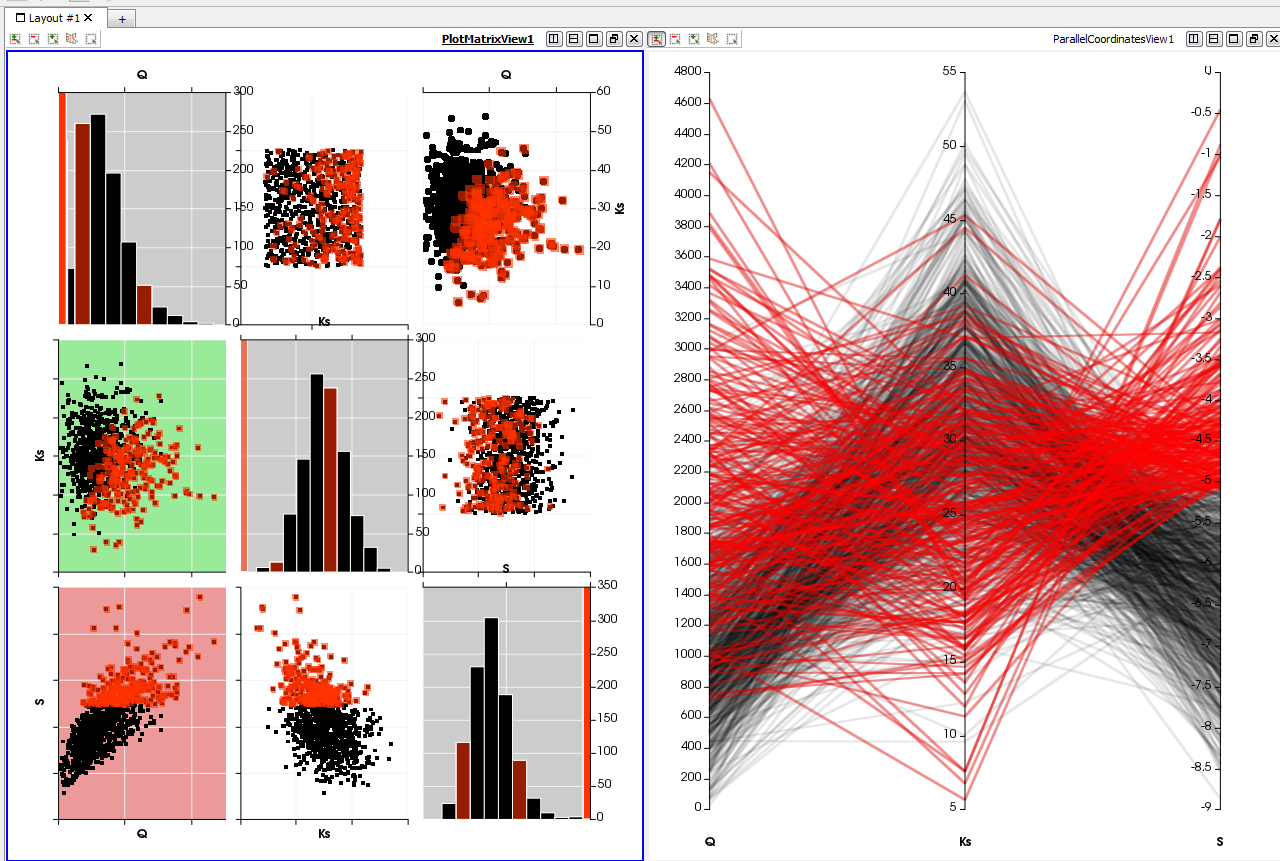
\includegraphics[width=0.9\textwidth]{figures/image032.png}
\end{center}

\end{frame}

%%%%%%%%%%%%%%%%%%%%%%%%%%%%%%%%%%%%%%%%%%%%%%%%%%%%%%%%%%%%%%%%%%%%%%%%%%%%%

\begin{frame}
\frametitle{Methodology}

\begin{center}
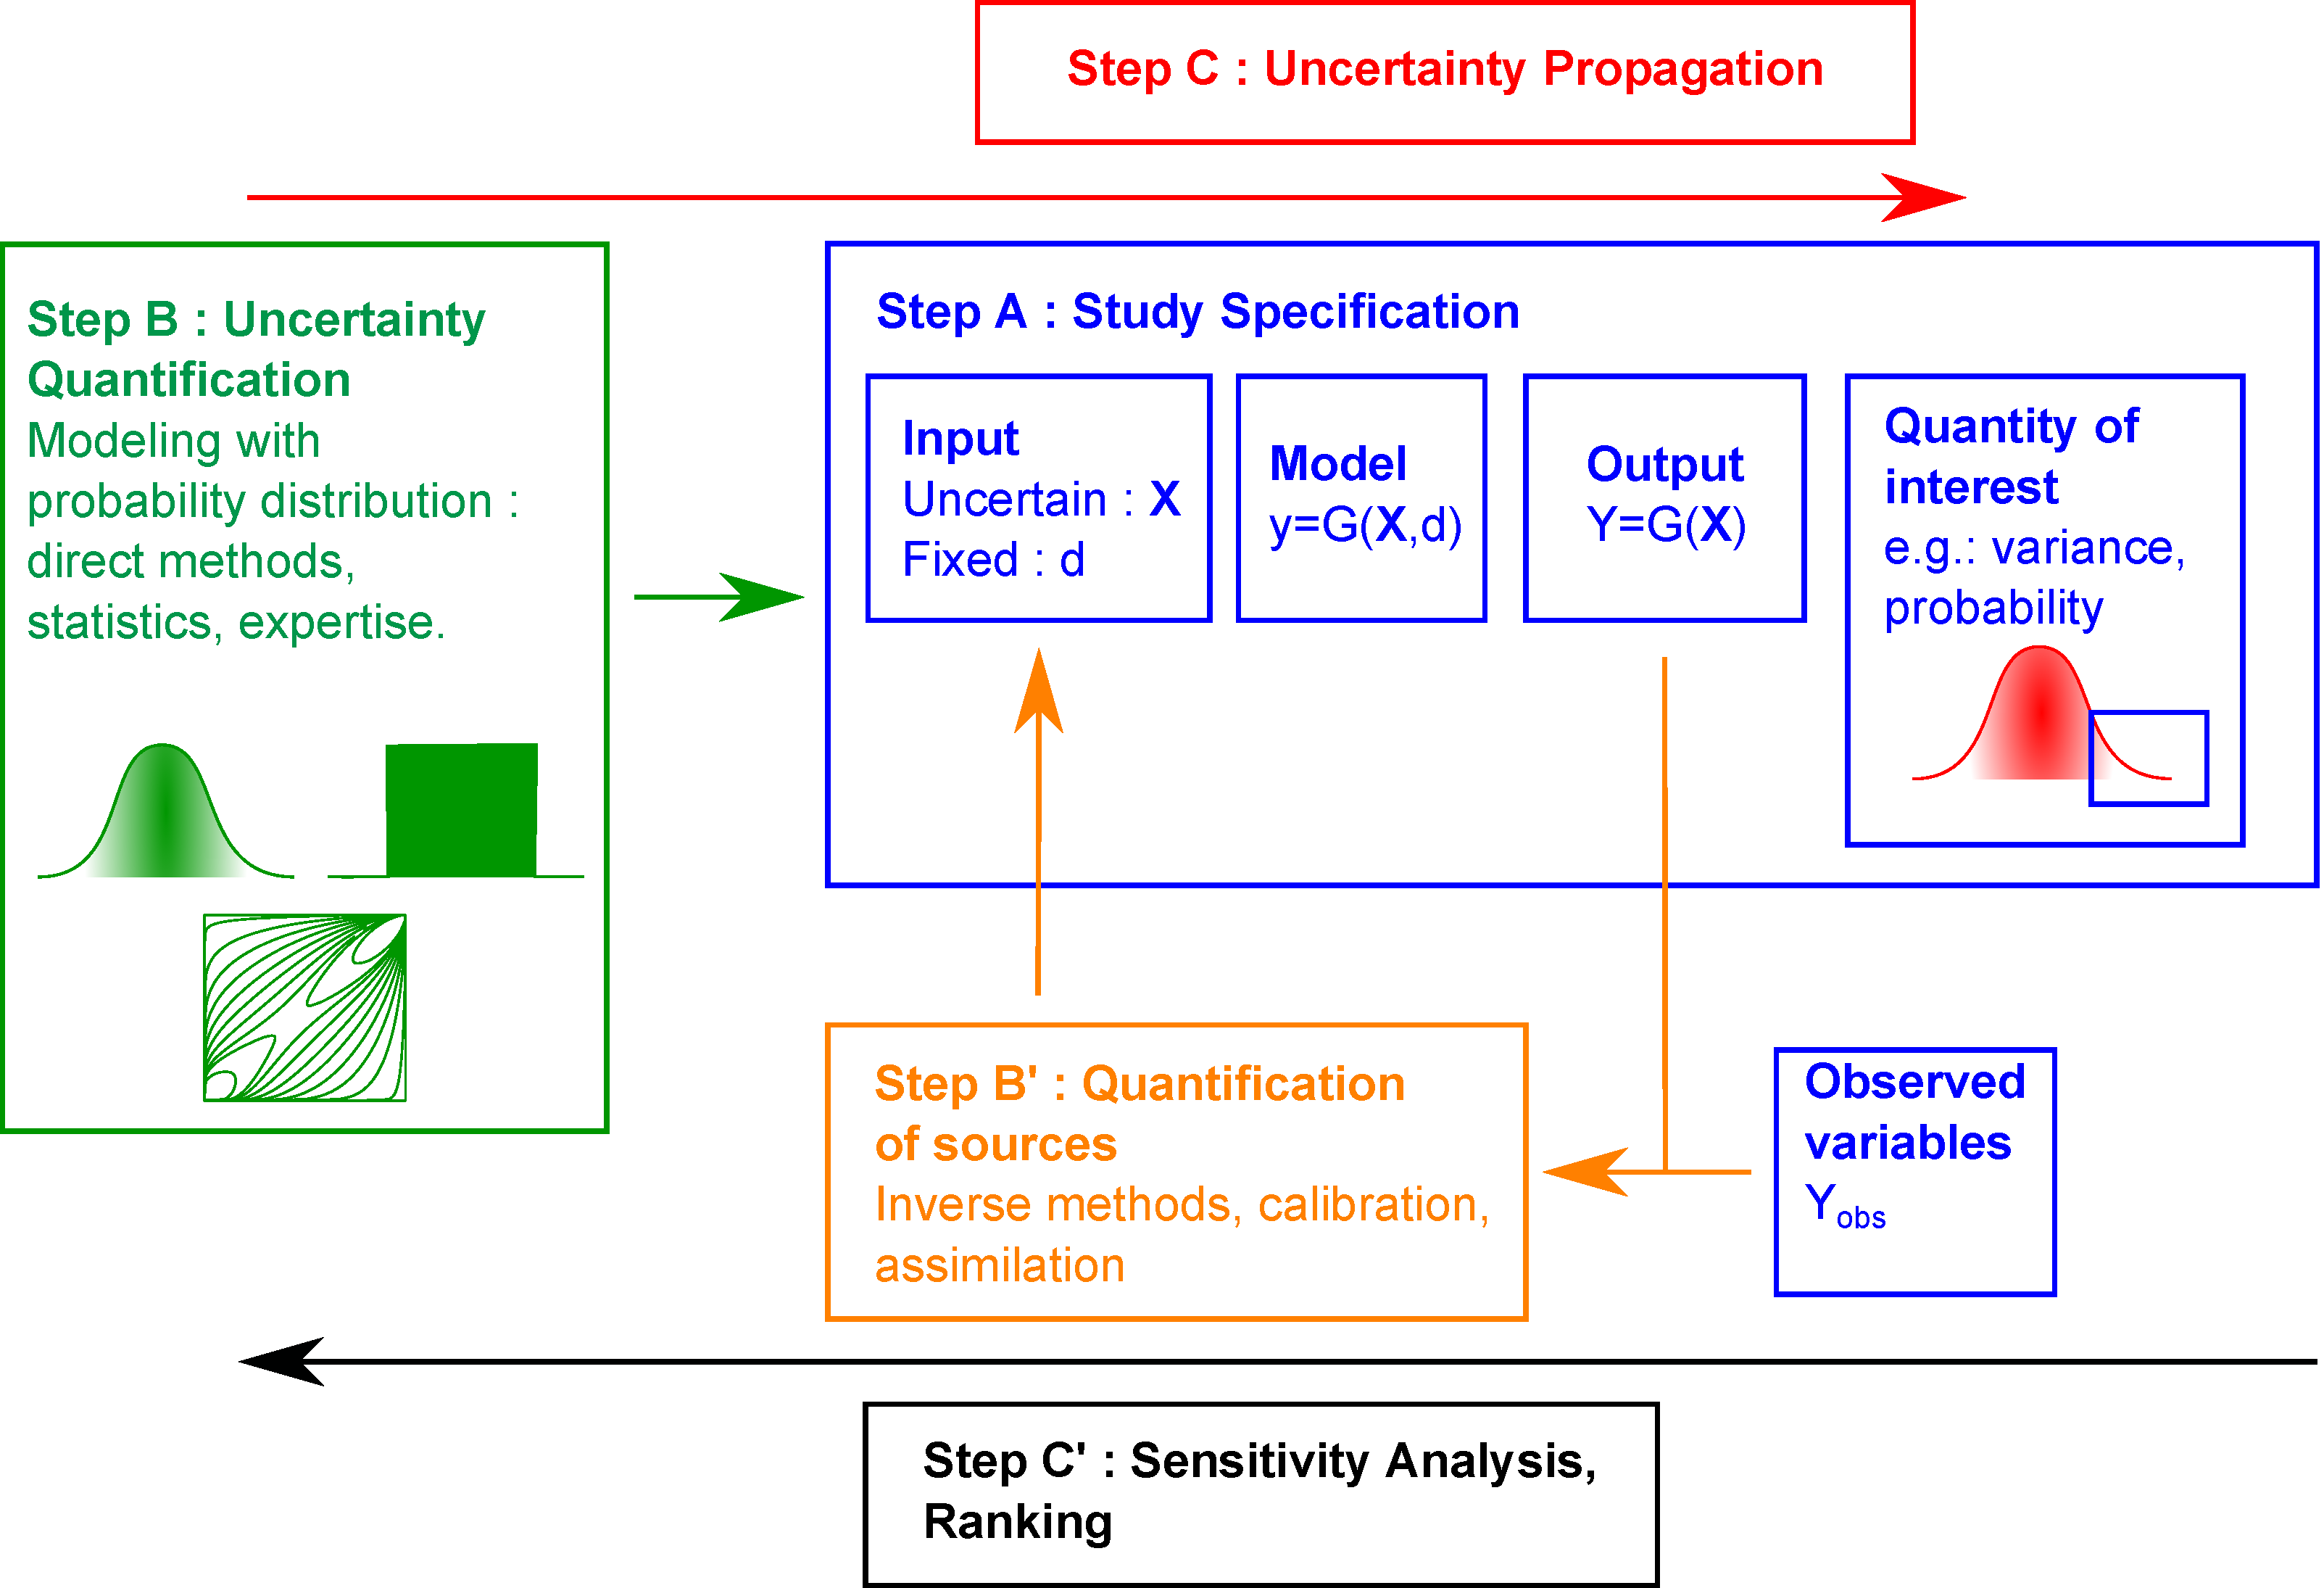
\includegraphics[width=0.9\textwidth]{figures/MethodologieIncertitude-EN.pdf}
\end{center}

\end{frame}

%%%%%%%%%%%%%%%%%%%%%%%%%%%%%%%%%%%%%%%%%%%%%%%%%%%%%%%%%%%%%%%%%%%%%%%%%%%%%

\begin{frame}
\frametitle{Software architecture}

  \begin{columns}
    \column{0.4\textwidth}
	
Two entry points:
\begin{itemize}
\item interactive,
\item Python.
\end{itemize}

Advantages of the Python programming of the GUI:
\begin{itemize}
\item unit tests,
\item going beyond the GUI
\end{itemize}

    \column{0.6\textwidth}

\begin{center}
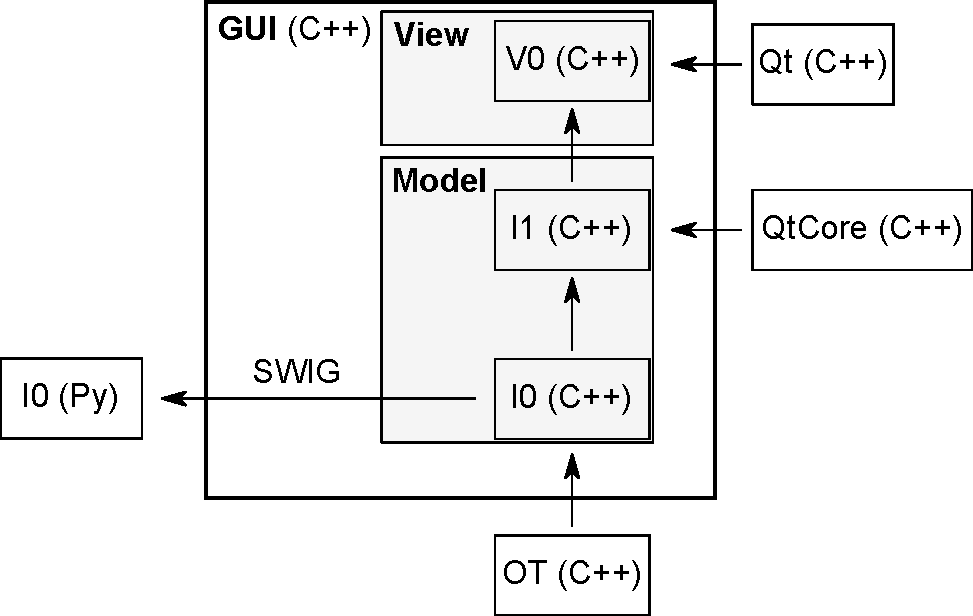
\includegraphics[width=0.95\textwidth]{figures/ArchiGUI-Internal.pdf}
\end{center}

	\end{columns}

\begin{center}
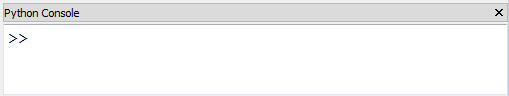
\includegraphics[width=0.9\textwidth]{figures/image007.png}
\end{center}

\end{frame}

%%%%%%%%%%%%%%%%%%%%%%%%%%%%%%%%%%%%%%%%%%%%%%%%%%%%%%%%%%%%%%%%%%%%%%%%%%%%%
%\section{Demo backup}

%%%%%%%%%%%%%%%%%%%%%%%%%%%%%%%%%%%%%%%%%%%%%%%%%%%%%%%%%%%%%%%%%%%%%%%%%%%%%

\begin{frame}
\frametitle{Symbolic physical model}

\begin{center}
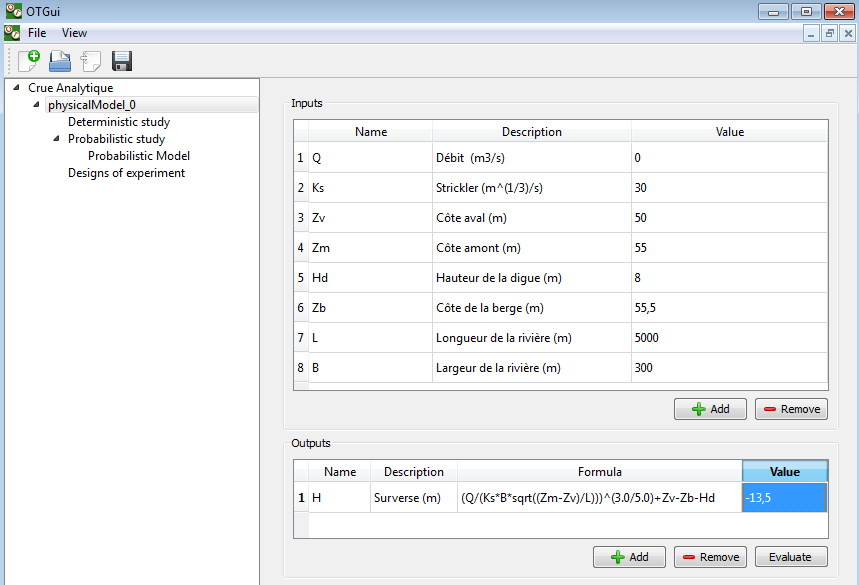
\includegraphics[width=0.9\textwidth]{figures/image009.png}
\end{center}

\end{frame}

%%%%%%%%%%%%%%%%%%%%%%%%%%%%%%%%%%%%%%%%%%%%%%%%%%%%%%%%%%%%%%%%%%%%%%%%%%%%%

\begin{frame}
\frametitle{Probabilistic model}

\begin{center}
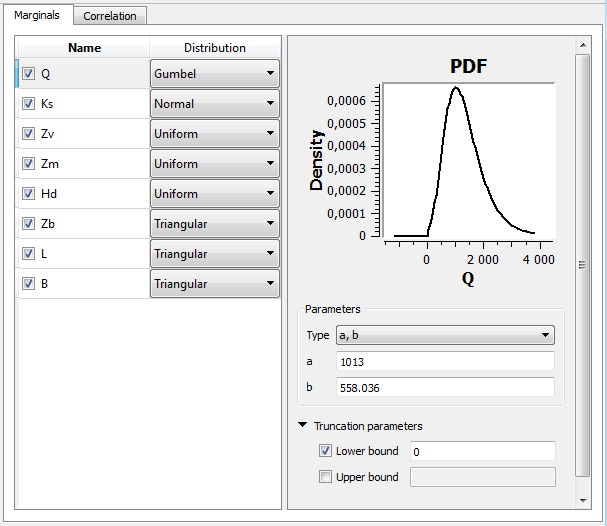
\includegraphics[height=0.8\textheight]{figures/image013.png}
\end{center}

\end{frame}

%%%%%%%%%%%%%%%%%%%%%%%%%%%%%%%%%%%%%%%%%%%%%%%%%%%%%%%%%%%%%%%%%%%%%%%%%%%%%

\begin{frame}
\frametitle{Limit state study : definition of the threshold}

\begin{center}
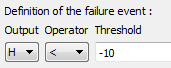
\includegraphics[width=0.4\textwidth]{figures/image015.png}
\end{center}

\end{frame}

%%%%%%%%%%%%%%%%%%%%%%%%%%%%%%%%%%%%%%%%%%%%%%%%%%%%%%%%%%%%%%%%%%%%%%%%%%%%%

\begin{frame}
\frametitle{Limit state study : algorithm parameters}

\begin{center}
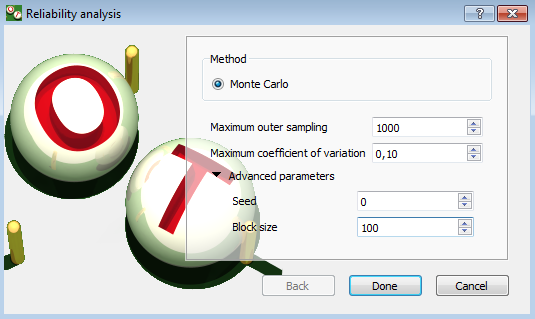
\includegraphics[width=0.95\textwidth]{figures/image017.png}
\end{center}

\end{frame}

%%%%%%%%%%%%%%%%%%%%%%%%%%%%%%%%%%%%%%%%%%%%%%%%%%%%%%%%%%%%%%%%%%%%%%%%%%%%%

\begin{frame}
\frametitle{Limit state study : summary}

\begin{center}
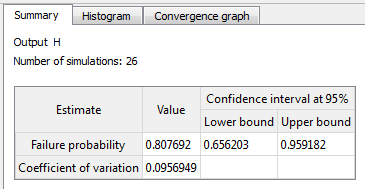
\includegraphics[width=0.7\textwidth]{figures/image019.png}
\end{center}

\end{frame}

%%%%%%%%%%%%%%%%%%%%%%%%%%%%%%%%%%%%%%%%%%%%%%%%%%%%%%%%%%%%%%%%%%%%%%%%%%%%%

\begin{frame}
\frametitle{Limit state study : histogram}

\begin{center}
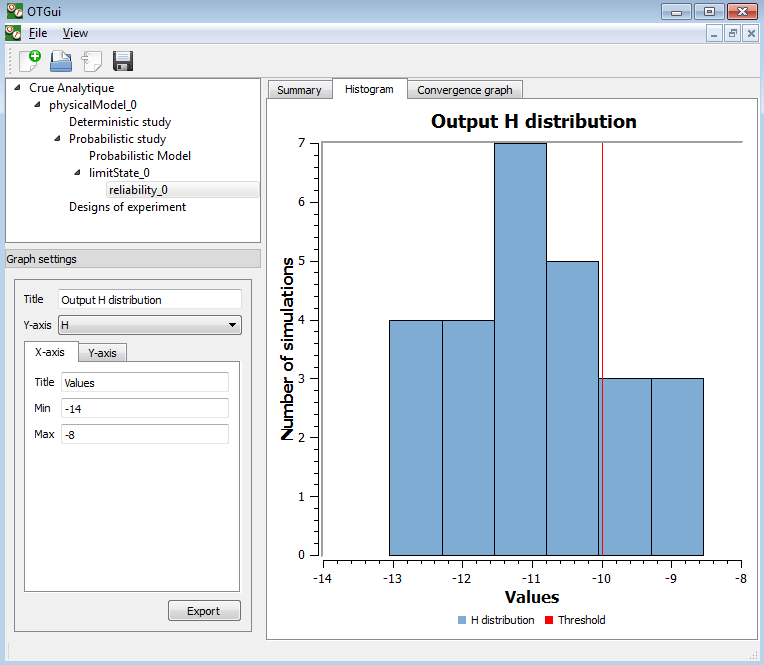
\includegraphics[width=0.7\textwidth]{figures/image021.png}
\end{center}

\end{frame}

%%%%%%%%%%%%%%%%%%%%%%%%%%%%%%%%%%%%%%%%%%%%%%%%%%%%%%%%%%%%%%%%%%%%%%%%%%%%%

\begin{frame}
\frametitle{Central tendency : algorithm parameters}

\begin{center}
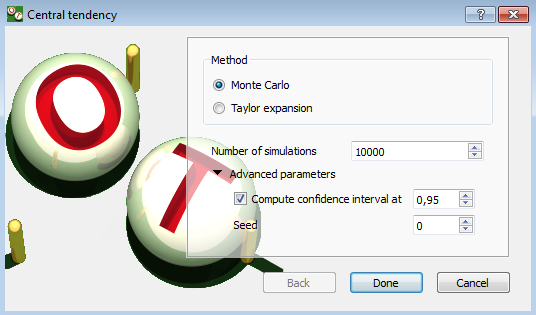
\includegraphics[width=0.8\textwidth]{figures/image023.png}
\end{center}

\end{frame}

%%%%%%%%%%%%%%%%%%%%%%%%%%%%%%%%%%%%%%%%%%%%%%%%%%%%%%%%%%%%%%%%%%%%%%%%%%%%%

\begin{frame}
\frametitle{Central tendency : summary results}

\begin{center}
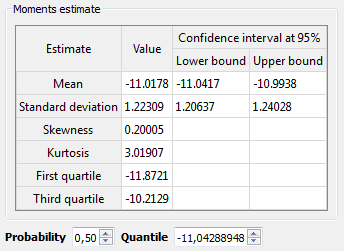
\includegraphics[width=0.8\textwidth]{figures/image025-bottom.png}
\end{center}

\end{frame}

%%%%%%%%%%%%%%%%%%%%%%%%%%%%%%%%%%%%%%%%%%%%%%%%%%%%%%%%%%%%%%%%%%%%%%%%%%%%%

\begin{frame}
\frametitle{Central tendency : summary results}

\begin{center}
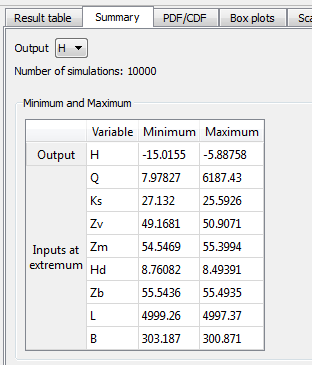
\includegraphics[height=0.8\textheight]{figures/image025-top.png}
\end{center}

\end{frame}

%%%%%%%%%%%%%%%%%%%%%%%%%%%%%%%%%%%%%%%%%%%%%%%%%%%%%%%%%%%%%%%%%%%%%%%%%%%%%

\begin{frame}
\frametitle{Central tendency : scatter plots}

\begin{center}
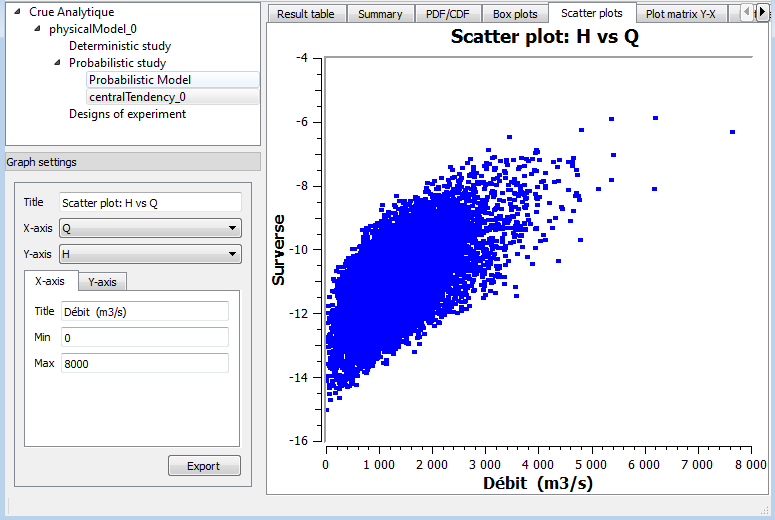
\includegraphics[width=0.8\textwidth]{figures/image028.png}
\end{center}

\end{frame}


%%%%%%%%%%%%%%%%%%%%%%%%%%%%%%%%%%%%%%%%%%%%%%%%%%%%%%%%%%%%%%%%%%%%%%%%%%%%%

\begin{frame}
\frametitle{Sensitivity analysis : Sobol' indices}

\begin{center}
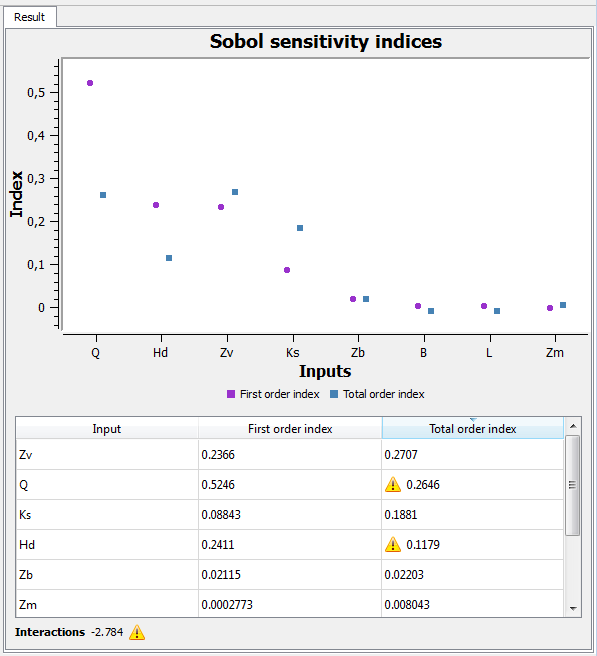
\includegraphics[height=0.8\textheight]{figures/image030.png}
\end{center}

\end{frame}

% %%%%%%%%%%%%%%%%%%%%%%%%%%%%%%%%%%%%%%%%%%%%%%%%%%%%%%%%%%%%%%%%%%%%%%%%%%%%%

\begin{frame}[containsverbatim]
\frametitle{OpenTURNS: estimate the mean}

See the Jupyter Notebook.

\scriptsize{

\lstset{language=python}
\begin{lstlisting}
from openturns.viewer import View
import openturns as ot
from math import sqrt

ot.RandomGenerator.SetSeed(0)

# 1. The function G
def functionCrue(X) :
    Q, Ks, Zv, Zm = X
    alpha = (Zm - Zv)/5.0e3
    H = (Q/(Ks*300.0*sqrt(alpha)))**(3.0/5.0)
    S = [H + Zv - (55.5 + 3.0)]
    return S

# Creation of the problem function
g = ot.PythonFunction(4, 1, functionCrue) 
g = ot.MemoizeFunction(g)
\end{lstlisting}

}

\end{frame}

% %%%%%%%%%%%%%%%%%%%%%%%%%%%%%%%%%%%%%%%%%%%%%%%%%%%%%%%%%%%%%%%%%%%%%%%%%%%%%

\begin{frame}[containsverbatim]
\frametitle{OpenTURNS: estimate the mean}

\begin{columns}
    \column{0.65\textwidth}

\scriptsize{

\lstset{language=python}
\begin{lstlisting}
# 2. Random vector definition
myParamQ = ot.GumbelAB(1013., 558.)
Q = ot.ParametrizedDistribution(myParamQ)
otLOW = ot.TruncatedDistribution.LOWER
Q = ot.TruncatedDistribution(Q, 0, otLOW)
Ks = ot.Normal(30.0, 7.5)
Ks = ot.TruncatedDistribution(Ks, 0, otLOW)
Zv = ot.Uniform(49.0, 51.0)
Zm = ot.Uniform(54.0, 56.0)

# 3. View the PDF
Q.setDescription(["Q (m3/s)"])
View(Q.drawPDF()).show()
\end{lstlisting}

}

\column{0.35\textwidth}
	\begin{center}
	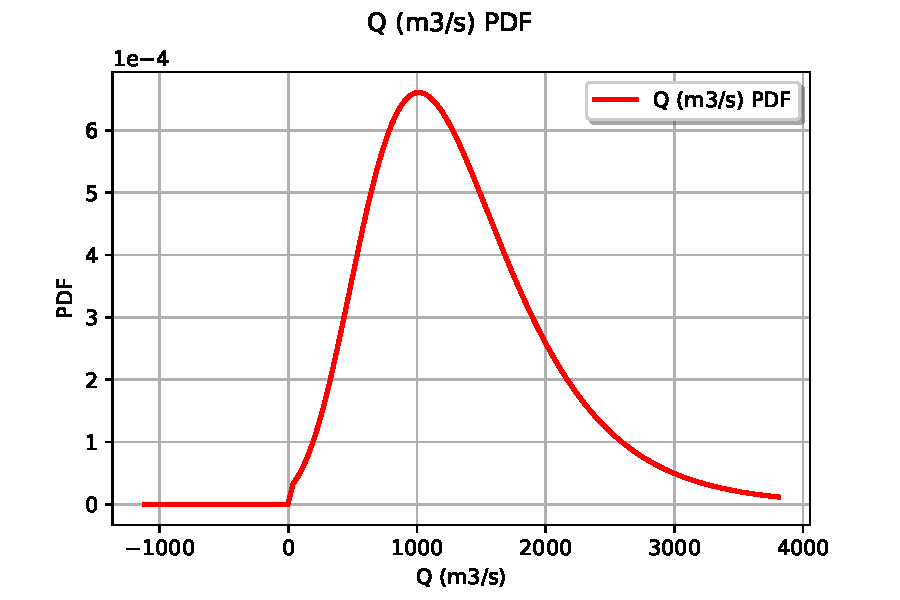
\includegraphics[width=0.95\textwidth]{figures/Q.pdf}
	\end{center}


\end{columns}

\end{frame}

% %%%%%%%%%%%%%%%%%%%%%%%%%%%%%%%%%%%%%%%%%%%%%%%%%%%%%%%%%%%%%%%%%%%%%%%%%%%%%

\begin{frame}[containsverbatim]
\frametitle{OpenTURNS: estimate the mean}


\scriptsize{

\lstset{language=python}
\begin{lstlisting}
# 4. Create the joint distribution function, 
#    the output and the event. 
X = ot.ComposedDistribution([Q, Ks, Zv, Zm])
Y = ot.RandomVector(g, ot.RandomVector(X))

# 5. Estimate expectation with simple Monte-Carlo
sampleSize = 10000
sampleX = X.getSample(sampleSize)
sampleY = g(sampleX)
sampleMean = sampleY.computeMean()
print("Mean=%f" % (sampleMean[0]))
\end{lstlisting}

Output: 
\begin{lstlisting}
Mean by MC =-5.937845
\end{lstlisting}

}

\end{frame}

%%%%%%%%%%%%%%%%%%%%%%%%%%%%%%%%%%%%%%%%%%%%%%%%%%%%%%%%%%%%%%%%%%%%%%%%%%%%%

%\section{Demo}

\begin{frame}
\frametitle{GUI : the demo}

\begin{center}
Demo time.
\end{center}

\end{frame}

%%%%%%%%%%%%%%%%%%%%%%%%%%%%%%%%%%%%%%%%%%%%%%%%%%%%%%%%%%%%%%%%%%%%%%%%%%%%%


\begin{frame}
\frametitle{GUI : outline}

\begin{itemize}
\item From scratch : 3 inputs, 2 outputs, sum, central dispersion study with default parameters
\item Open axialStressedBeam-python.xml : central dispersion with sample size 1000, Threshold P(G<0) with CV=0.05
\item Import crue-4vars-analytique.py : S.A. with sample size 1000, sort by size
\end{itemize}

\end{frame}


%%%%%%%%%%%%%%%%%%%%%%%%%%%%%%%%%%%%%%%%%%%%%%%%%%%%%%%%%%%%%%%%%%%%%%%%%%%%%
%\section{Background}

\begin{frame}
\frametitle{UQ, the easy way}

Main goal : make UQ easy to use
\begin{itemize}
\item classical user-friendly algorithms with a 
state-of-the-art implementation,
\item default parameters of the algorithms whenever possible,
\item an easy access to the HPC resources,
\item an automated connection to the computer code.
\end{itemize}

Produce standard results :
\begin{itemize}
\item numerical results e.g. tables,
\item classical graphics.
\end{itemize}

\end{frame}

%%%%%%%%%%%%%%%%%%%%%%%%%%%%%%%%%%%%%%%%%%%%%%%%%%%%%%%%%%%%%%%%%%%%%%%%%%%%%

\begin{frame}
\frametitle{Overview (1/2)}

Inputs from the user :
\begin{itemize}
\item Physical model : symbolic, Python code or SALOME component
\item Probabilistic model : joint probability distribution function of the input.
\end{itemize}

Then :
\begin{itemize}
\item Central dispersion: estimates the central dispersion of the output Y (e.g. mean).
\item Threshold probability: estimates the probability that the output exceeds a given
threshold S.
\item Sensitivity analysis: estimates the importance of the inputs to the variability of the output.
\end{itemize}

\end{frame}

%%%%%%%%%%%%%%%%%%%%%%%%%%%%%%%%%%%%%%%%%%%%%%%%%%%%%%%%%%%%%%%%%%%%%%%%%%%%%

\begin{frame}
\frametitle{Overview (2/2)}

Probabilistic modeling :
\begin{itemize}
\item Distribution fitting from a sample
\item Dependence modeling (Gaussian copula)
\end{itemize}

Meta-modeling :
\begin{itemize}
\item Polynomial chaos (full or sparse)
\item Kriging
\end{itemize}

\end{frame}



\end{document}
